\section*{ДОДАТОК~А. Повні результати кількісної апробації}

Нижче наведено результати Монте-Карло моделювання для реалістичного модельного українського ЗВО: 300~НПП, 20~кафедр (приблизно 5~факультетів), синтетичні дані без персональних записів. Усі методи оцінювалися на ідентичних входах; подано середнє\,$\pm$\,95\,\% довірчий інтервал за $K=30$ початковими значеннями генератора.

\subsection*{А.1. Якість дедуплікації}

\begin{table}[ht]
\centering
\caption{Якість дедуплікації, середнє\,$\pm$\,95\,\% довірчий інтервал, \%}
\label{tab:res-dedup}
\begin{tabular}{lcccc}
\toprule
Метод & $P$ & $R$ & $F_1$ & $B^3 F_1$ \\
\midrule
DOI-only        & $100{,}0 \pm 0{,}0$ & $42{,}6 \pm 0{,}5$ & $59{,}7 \pm 0{,}5$ & $93{,}7 \pm 0{,}1$ \\
Title+Year      & $83{,}3 \pm 0{,}6$  & $39{,}4 \pm 0{,}4$ & $53{,}5 \pm 0{,}4$ & $92{,}7 \pm 0{,}1$ \\
Fuzzy (незважений) & $83{,}7 \pm 0{,}6$ & $41{,}1 \pm 0{,}4$ & $55{,}1 \pm 0{,}4$ & $92{,}9 \pm 0{,}1$ \\
\textbf{Golden Record} & $\mathbf{88{,}2 \pm 0{,}5}$ & $\mathbf{68{,}1 \pm 0{,}6}$ & $\mathbf{76{,}8 \pm 0{,}4}$ & $\mathbf{95{,}8 \pm 0{,}1}$ \\
\bottomrule
\end{tabular}
\end{table}

Golden Record домінує за $F_1$ та повнотою: довірчий інтервал $F_1$ ($[76{,}4; 77{,}2]$) не перетинається з інтервалами базових методів. DOI-only очікувано має $P=100\,\%$, але пропускає більшість дублікатів без DOI; Title+Year вразливий до перекладів, транслітерації й колізій назв. Показово, що незважений нечіткий зіставлювач (Fuzzy) на тих самих ознаках дає лише $F_1 = 55{,}1\,\%$ --- ненабагато вище за Title+Year і значно нижче за Golden Record: отже виграш зумовлений не самим фактом використання нечіткої подібності, а \textit{зваженим логістичним} зіставленням із DOI-свідченням та охоронцем конфлікту DOI. Кластерна метрика $B^3 F_1$ висока й близька для всіх методів (92--96\,\%), бо корпус домінують одиничні кластери (більшість праць не дублюються); тому розрізнювальною метрикою якості дедуплікації є саме парний $F_1$, а не $B^3$. Порівняння методів показано на рис.~\ref{fig:res-method}.

\begin{figure}[ht]
\centering
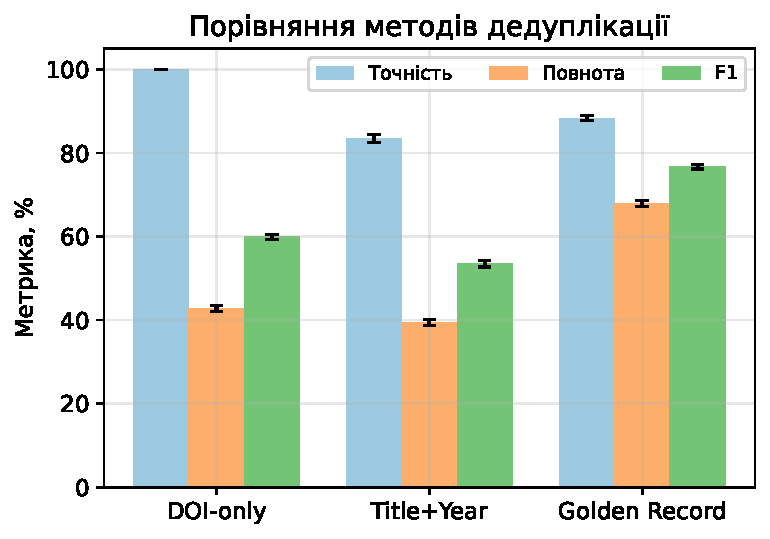
\includegraphics[width=0.8\linewidth]{../figures/f3_method_comparison.pdf}
\caption{Порівняння методів дедуплікації за точністю, повнотою та $F_1$.}
\label{fig:res-method}
\end{figure}

\subsection*{А.2. Чутливість конвеєра}

За зміни частки дублювання від 10\,\% до 30\,\% $F_1$ Golden Record становить відповідно 70,2\,\%, 74,0\,\%, 76,3\,\%, 78,2\,\% і 78,9\,\% (рис.~\ref{fig:res-dup}). Впорядкування методів зберігається, отже висновок не залежить від одного припущення про рівень фрагментації.

\begin{figure}[ht]
\centering
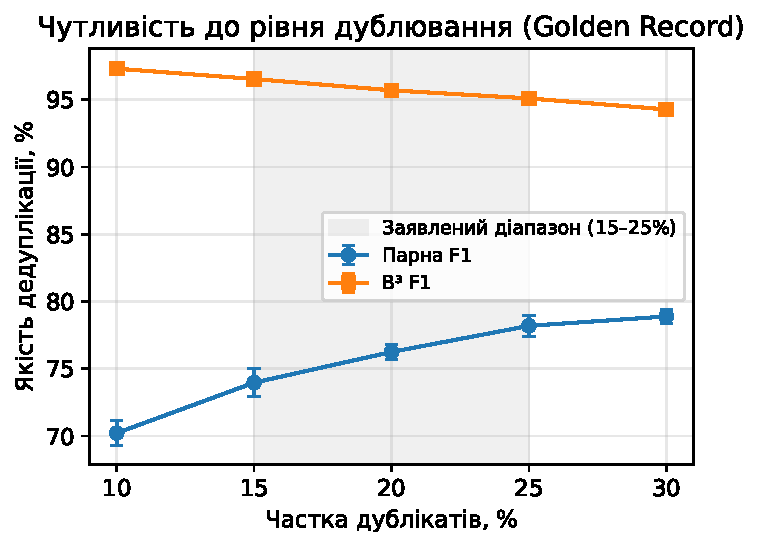
\includegraphics[width=0.8\linewidth]{../figures/f1_dup_sensitivity.pdf}
\caption{Чутливість $F_1$ Golden Record до частки дублювання записів (10--30\,\%).}
\label{fig:res-dup}
\end{figure}

За зростання множника спотворення метаданих точність деградує плавно: $P=91{,}6\,\%$, 89,6\,\%, 87,5\,\%, 83,9\,\%, 81,2\,\%; повнота падає різкіше: $R=80{,}9\,\%$, 76,0\,\%, 67,6\,\%, 58,8\,\%, 50,9\,\% (рис.~\ref{fig:res-corr}). Такий режим є прийнятним для звітності: за сильного шуму система радше пропускає злиття, ніж хибно об'єднує різні праці.

\begin{figure}[ht]
\centering
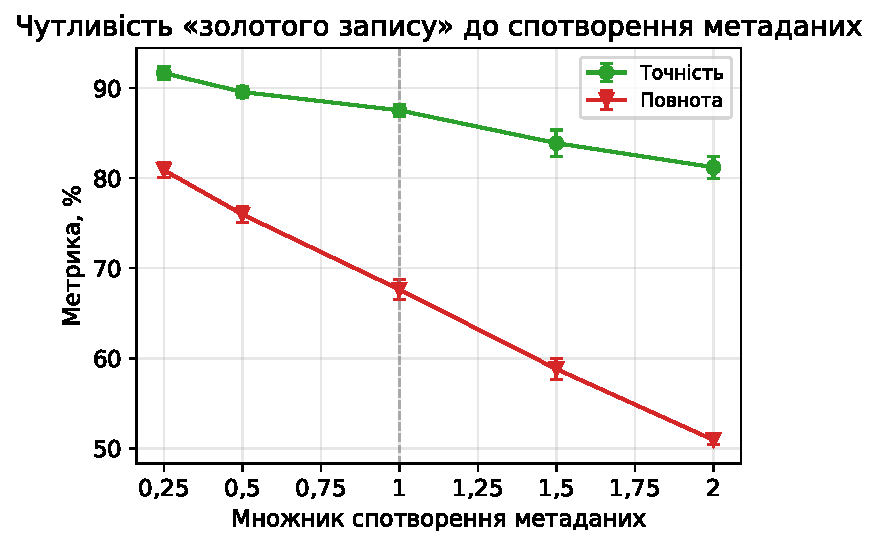
\includegraphics[width=0.8\linewidth]{../figures/f2_corruption_sensitivity.pdf}
\caption{Чутливість точності та повноти до множника спотворення метаданих (0,25--2,0).}
\label{fig:res-corr}
\end{figure}

\subsection*{А.3. Якість полів та ефективність}

\begin{table}[ht]
\centering
\caption{Повнота та точність полів злитого золотого запису, \%}
\label{tab:res-fields}
\begin{tabular}{lc}
\toprule
Показник поля & Значення \\
\midrule
Наявність DOI (DOI present)   & $45{,}4 \pm 0{,}4$ \\
Коректність DOI (DOI correct) & $67{,}8 \pm 0{,}2$ \\
Точність року (Year accuracy) & $80{,}9 \pm 0{,}2$ \\
Точність назви (Title accuracy) & $99{,}95 \pm 0{,}01$ \\
\bottomrule
\end{tabular}
\end{table}

Майже досконала точність назви підтверджує ефект виправлення Unicode-нормалізатора: стара процедура знищувала 100\,\% україномовних назв, що блокувало зіставлення за назвою саме для кириличного корпусу.

\begin{table}[ht]
\centering
\caption{Ефективність: рушій (виміряно) проти аналітичної моделі ручної праці}
\label{tab:res-eff}
\begin{tabular}{ll}
\toprule
Показник & Значення \\
\midrule
Середня кількість записів на ЗВО & $\approx 7056$ \\
Середня кількість рішень дедуплікації & $\approx 1441$ \\
Час рушія (дедуплікація+злиття, весь ЗВО) & $1{,}58 \pm 0{,}15$\,с \\
Модель ручної праці (на ЗВО, рік) & $\approx 429{,}1$\,год \\
Модель ручної праці (на кафедральний звіт) & $\approx 21{,}45$\,год \\
Смуга HITL (на дослідника) & $\approx 56{,}5$\,пар \\
\bottomrule
\end{tabular}
\end{table}

Час рушія охоплює лише обчислення дедуплікації та злиття, без мережевих запитів до ORCID/OpenAlex/Scopus. Ручна трудомісткість є прозорою аналітичною моделлю $\text{manual}=a\cdot\text{записи}+b\cdot\text{рішення\_дедуплікації}+c$, де $a=2{,}5$ хв/запис, $b=5$ хв/рішення, $c=45$ хв/звіт. Коефіцієнти не подаються як хронометражне дослідження; це відтворюваний сценарій, калібрований за декомпозицією операцій звітності та узгоджений із зовнішніми даними про значне адміністративне навантаження науковців \cite{Rockwell2009FDPBurden}. Для сценарію 300~НПП автоматизована частка цієї моделі становить близько 96,5\,\%, але невизначені пари лишаються в контурі HITL.
